
\section{Polylines}
\label{sec:org642cdb8}
\lstset{language=r,label= ,caption= ,captionpos=b,numbers=none}
\begin{lstlisting}
load('data/CO2.RData')
\end{lstlisting}

\index{Data!CO2@$CO_2$}
\index{Data!World Bank}

Our first approach is to display the entire data in a panel with a
scatterplot using country names as the grouping factor. Points of each
country are connected with polylines to reveal the time evolution
(Figure \ref{fig:CO2-GNI}).
\lstset{language=r,label= ,caption= ,captionpos=b,numbers=none}
\begin{lstlisting}
## lattice version
xyplot(GNI.capita  ~ CO2.capita, data=CO2data,
       xlab="Carbon dioxide emissions (metric tons per capita)",
       ylab="GNI per capita, PPP (current international $)",
       groups=Country.Name, type='b')
\end{lstlisting}

\begin{figure}[htbp]
\centering
\includegraphics[width=.9\linewidth]{figs/CO2_GNI.pdf}
\caption{GNI per capita versus \(\mathrm{CO_2}\) emissions per capita (\texttt{lattice} version). \label{fig:CO2-GNI}}
\end{figure}

\lstset{language=r,label= ,caption= ,captionpos=b,numbers=none}
\begin{lstlisting}
## ggplot2 version
ggplot(data=CO2data, aes(x=CO2.capita, y=GNI.capita,
                         color=Country.Name)) +
    xlab("Carbon dioxide emissions (metric tons per capita)") +
    ylab("GNI per capita, PPP (current international $)") +
    geom_point() + geom_path() + theme_bw()
\end{lstlisting}

Three improvements can be added to this graphical result: 
\begin{enumerate}
\item Define a better palette to enhance visual discrimination between
countries.
\item Display time information with labels to show year values.
\item Label each polyline with the country name instead of a legend.
\end{enumerate}

\section{Choosing Colors}
\label{sec:org89622e3}
The \texttt{Country.Name} categorical variable will be encoded with a
qualitative palette, namely the first five colors of \texttt{Set1}
palette\footnote{\url{http://colorbrewer2.org/}} from the \texttt{RColorBrewer} package
\cite{Neuwirth2011}. Because there are more countries than colors, we
have to repeat some colors to complete the number of levels of the
variable \texttt{Country.Name}. The result is a palette with non-unique
colors, and thus some countries will share the same color. This is not
a problem because the curves will be labeled, and countries with the
same color will be displayed at enough distance.

\index{Packages!RColorBrewer@\texttt{RColorBrewer}}
\index{brewer.pal@\texttt{brewer.pal}}

\lstset{language=r,label= ,caption= ,captionpos=b,numbers=none}
\begin{lstlisting}
library(RColorBrewer)

nCountries <- nlevels(CO2data$Country.Name)
pal <- brewer.pal(n=5, 'Set1')
pal <- rep(pal, length = nCountries)
\end{lstlisting}

Adjacent colors of this palette are chosen to be easily
distinguishable. Therefore, the connection between colors and
countries must be in such a way that nearby lines are encoded
with adjacent colors of the palette.

A simple approach is to calculate the annual average of the
variable to be represented along the x-axis (\texttt{CO2.capita}), and
extract colors from the palette according to the order of this
value.  

\index{aggregate@\texttt{aggregate}}

\lstset{language=r,label= ,caption= ,captionpos=b,numbers=none}
\begin{lstlisting}
## Rank of average values of CO2 per capita
CO2mean <- aggregate(CO2.capita ~ Country.Name, data=CO2data, FUN=mean)
palOrdered <- pal[rank(CO2mean$CO2.capita)]  
\end{lstlisting}

A more sophisticated solution is to use the ordered results of a
hierarchical clustering of the time evolution of the \(\mathrm{CO_2}\) per capita
values (Figure \ref{fig:hclustCO2}). The data is extracted from the
original \(\mathrm{CO_2}\) \texttt{data.frame}.  

\index{hclust@\texttt{hclust}}

\lstset{language=r,label= ,caption= ,captionpos=b,numbers=none}
\begin{lstlisting}
CO2capita <- CO2data[, c('Country.Name',
                         'Year',
                         'CO2.capita')]
CO2capita <- reshape(CO2capita,
                     idvar='Country.Name',
                     timevar='Year',
                     direction='wide')
hCO2 <- hclust(dist(CO2capita[, -1]))

oldpar <- par(mar=c(0, 2, 0, 0) + .1)
plot(hCO2, labels=CO2capita$Country.Name,
     xlab='', ylab='', sub='', main='')
par(oldpar)
\end{lstlisting}

\begin{figure}[htbp]
\centering
\includegraphics[width=.9\linewidth]{figs/hclust.pdf}
\caption{Hierarchical clustering of the time evolution of \(\mathrm{CO_2}\) per capita values. \label{fig:hclustCO2}}
\end{figure}


The colors of the palette are assigned to each country with \texttt{match},
which returns a vector of the positions of the matches of the country
names in alphabetical order in the country names ordered according to
the hierarchical clustering.
\lstset{language=r,label= ,caption= ,captionpos=b,numbers=none}
\begin{lstlisting}
idx <- match(levels(CO2data$Country.Name), 
             CO2capita$Country.Name[hCO2$order])
palOrdered <- pal[idx]  
\end{lstlisting}
It must be highlighted that this palette links colors with the levels
of \texttt{Country.Name} (country names in alphabetical order), which is
exactly what the \texttt{groups} argument provides. The following code
produces a curve for each country using different colors to
distinguish them.

\index{simpleTheme@\texttt{simpleTheme}}
\lstset{language=r,label= ,caption= ,captionpos=b,numbers=none}
\begin{lstlisting}
## simpleTheme encapsulates the palette in a new theme for xyplot
myTheme <- simpleTheme(pch=19, cex=0.6, col=palOrdered)

pCO2.capita <- xyplot(GNI.capita  ~ CO2.capita,
                      data = CO2data,
                      xlab = "Carbon dioxide emissions (metric tons per capita)",
                      ylab = "GNI per capita, PPP (current international $)",
                      groups = Country.Name,
                      par.settings = myTheme,
                      type='b')
\end{lstlisting}

\lstset{language=r,label= ,caption= ,captionpos=b,numbers=none}
\begin{lstlisting}
gCO2.capita <- ggplot(data = CO2data,
                      aes(x = CO2.capita,
                          y = GNI.capita,
                          color = Country.Name)) +
    geom_point() + geom_path() +
    scale_color_manual(values=palOrdered, guide=FALSE) +
    xlab('CO2 emissions (metric tons per capita)') +
    ylab('GNI per capita, PPP (current international $)') +
    theme_bw()
\end{lstlisting}

\section{Labels to Show Time Information}
\label{sec:org8215fc3}
This result can be improved with labels displaying the years to show
the time evolution.  A panel function with \texttt{panel.text} to print the
year labels and \texttt{panel.superpose} to display the lines for each group
is a solution. In the panel function, \texttt{subscripts} is a vector with
the integer indices representing the rows of the \texttt{data.frame} to be
displayed in the panel.

\index{panel.text@\texttt{panel.text}}
\index{subscripts@\texttt{subscripts}}
\index{Panel function}
\index{panel.superpose@\texttt{panel.superpose}}


\lstset{language=r,label= ,caption= ,captionpos=b,numbers=none}
\begin{lstlisting}
xyplot(GNI.capita  ~ CO2.capita,
       data = CO2data
       xlab = "Carbon dioxide emissions (metric tons per capita)",
       ylab = "GNI per capita, PPP (current international $)",
       groups = Country.Name,
       par.settings = myTheme,
       type='b',
       panel = function(x, y, ..., subscripts, groups){
           panel.text(x, y, ...,
                      labels = CO2data$Year[subscripts],
                      pos = 2, cex = 0.5, col = 'gray')
           panel.superpose(x, y, subscripts, groups,...)
       })
\end{lstlisting}

The same result with a clearer code is obtained with the combination
of \texttt{+.trellis}, \texttt{glayer\_} and \texttt{panel.text}. Using \texttt{glayer\_} instead of
\texttt{glayer}, we ensure that the labels are printed below the lines.

\index{Packages!latticeExtra@\texttt{latticeExtra}}
\index{glayer@\texttt{glayer}}
\index{+.trellis@\texttt{+.trellis}}

\lstset{language=r,label= ,caption= ,captionpos=b,numbers=none}
\begin{lstlisting}
pCO2.capita <- pCO2.capita +
    glayer_(panel.text(...,
                       labels = CO2data$Year[subscripts],
                         pos = 2, cex = 0.5, col = 'gray'))
\end{lstlisting}

\lstset{language=r,label= ,caption= ,captionpos=b,numbers=none}
\begin{lstlisting}
gCO2.capita <- gCO2.capita + geom_text(aes(label = Year),
                                       colour = 'gray',
                                       size = 2.5,
                                       hjust = 0, vjust = 0)
  
\end{lstlisting}

\section{Country Names: Positioning Labels}
\label{sec:org974853f}
The common solution to link each curve with the group value is to add
a legend. However, a legend can be confusing with too many items. In
addition, the reader must carry out a complex task: Choose the line,
memorize its color, search for it in the legend, and read the country
name.

A better approach is to label each line using nearby text with the
same color encoding. A suitable method is to place the labels
close to the end of each line (Figure
\ref{fig:CO2-GNI-glayer}). Labels are placed with the
\texttt{panel.pointLabel} function from the \texttt{maptools} package. This
function use optimization routines to find locations without
overlaps.

\index{group.value@\texttt{group.value}}
\index{group.number@\texttt{group.number}}

\lstset{language=r,label= ,caption= ,captionpos=b,numbers=none}
\begin{lstlisting}
library(maptools)  
## group.value provides the country name; group.number is the index
## of each country to choose the color from the palette.
pCO2.capita +
    glayer(panel.pointLabel(mean(x), mean(y),
                            labels = group.value,
                            col = palOrdered[group.number],
                            cex = .8,
                            fontface = 2,
                            fontfamily = 'Palatino'))
\end{lstlisting}

\begin{figure}[htbp]
\centering
\includegraphics[width=.9\linewidth]{figs/CO2_capita.pdf}
\caption{\(\mathrm{CO_2}\) emissions versus GNI per capita. Labels are placed with \texttt{panel.pointLabel}. \label{fig:CO2-GNI-glayer}}
\end{figure}

However, this solution does not solve the overlapping between labels
and lines. The package \texttt{directlabels} \cite{Hocking2013} includes a
wide repertory of positioning methods to cope with this problem. The
main function, \texttt{direct.label}, is able to determine a suitable method
for each plot, although the user can choose a different method from
the collection or even define a custom method. For the \texttt{pCO2.capita}
object, I have obtained the best results with \texttt{extreme.grid} (Figure
\ref{fig:CO2-GNI-DL}).

\index{Packages!directlabels@\texttt{directlabels}}
\index{direct.label@\texttt{direct.label}}

\lstset{language=r,label= ,caption= ,captionpos=b,numbers=none}
\begin{lstlisting}
library(directlabels)

direct.label(pCO2.capita,
             method = 'extreme.grid')
\end{lstlisting}

\begin{figure}[htbp]
\centering
\includegraphics[width=.9\linewidth]{figs/CO2_capitaDL.pdf}
\caption{\(\mathrm{CO_2}\) emissions versus GNI per capita. Labels are placed with the \texttt{extreme.grid} method of the \texttt{directlabels} package. \label{fig:CO2-GNI-DL}}
\end{figure}

\lstset{language=r,label= ,caption= ,captionpos=b,numbers=none}
\begin{lstlisting}
direct.label(gCO2.capita, method='extreme.grid')
\end{lstlisting}

\section{A Panel for Each Year}
\label{sec:orga81495a}
Time can be used as a conditioning variable (as shown in previous
sections) to display subsets of the data in different panels. Figure
\ref{fig:CO2-GNI-panel} is produced with the same code as in Figure
\ref{fig:CO2-GNI}, now including \texttt{|factor(Year)} in the lattice
version and \texttt{facet\_wrap(\textasciitilde{} Year)} in the \texttt{ggplot2} version.

\lstset{language=r,label= ,caption= ,captionpos=b,numbers=none}
\begin{lstlisting}
xyplot(GNI.capita  ~ CO2.capita | factor(Year),
       data = CO2data,
       xlab = "Carbon dioxide emissions (metric tons per capita)",
       ylab = "GNI per capita, PPP (current international $)",
       groups = Country.Name, type = 'b',
       auto.key = list(space = 'right'))
\end{lstlisting}

\begin{figure}[htbp]
\centering
\includegraphics[width=.9\linewidth]{figs/CO2_capita_panel.pdf}
\caption{\(\mathrm{CO_2}\) emissions versus GNI per capita with a panel for each year. \label{fig:CO2-GNI-panel}}
\end{figure}

\lstset{language=r,label= ,caption= ,captionpos=b,numbers=none}
\begin{lstlisting}
ggplot(data = CO2data,
       aes(x = CO2.capita,
           y = GNI.capita,
           colour = Country.Name)) +
    facet_wrap(~ Year) + geom_point(pch = 19) + 
    xlab('CO2 emissions (metric tons per capita)') +
    ylab('GNI per capita, PPP (current international $)') +
    theme_bw()
\end{lstlisting}

Because the grouping variable, \texttt{Country.Name}, has many levels, the
legend is not very useful. Once again, point labeling is recommended
(Figure \ref{fig:CO2-GNI-panel-labels}).

\lstset{language=r,label= ,caption= ,captionpos=b,numbers=none}
\begin{lstlisting}
xyplot(GNI.capita  ~ CO2.capita | factor(Year),
       data = CO2data,
       xlab = "Carbon dioxide emissions (metric tons per capita)",
       ylab = "GNI per capita, PPP (current international $)",
       groups = Country.Name, type = 'b',
       par.settings = myTheme) + 
    glayer(panel.pointLabel(x, y,
                            labels = group.value,
                            col = palOrdered[group.number],
                            cex = 0.7))
\end{lstlisting}

\begin{figure}[htbp]
\centering
\includegraphics[width=.9\linewidth]{figs/CO2_capita_panel_labels.pdf}
\caption{\(\mathrm{CO_2}\) emissions versus GNI per capita with a panel for each year. \label{fig:CO2-GNI-panel-labels}}
\end{figure}

\subsection{\floweroneleft Using Variable Size to Encode an Additional Variable}
\label{sec:orgfd6cb66}
Instead of using simple points, we can display circles of
different radius to encode a new variable. This new variable is
\texttt{CO2.PPP}, the ratio of \(\mathrm{CO_2}\) emissions to the Gross Domestic
Product with purchasing power parity (PPP) estimations.

To use this numeric variable as an additional grouping factor, its range must be divided into different classes. The typical solution is to use \texttt{cut} to coerce the numeric variable into a \texttt{factor} whose levels correspond to uniform intervals, which could be unrelated to the data distribution. The \texttt{classInt} package \cite{Bivand2013} provides several methods to partition data into classes based on natural groups in the data distribution.

\index{Packages!classInt@\texttt{classInt}}
\index{classIntervals@\texttt{classIntervals}}

\lstset{language=r,label= ,caption= ,captionpos=b,numbers=none}
\begin{lstlisting}
library(classInt)
z <- CO2data$CO2.PPP
intervals <- classIntervals(z, n = 4, style = 'fisher')
\end{lstlisting}

Although the functions of this package are mainly intended to create color palettes for maps, the results can also be associated to point sizes. \texttt{cex.key} defines the sequence of sizes (to be displayed in the legend) associated with each \texttt{CO2.PPP} using the \texttt{findCols} function.
\lstset{language=r,label= ,caption= ,captionpos=b,numbers=none}
\begin{lstlisting}
nInt <- length(intervals$brks) - 1
cex.key <- seq(0.5, 1.8, length = nInt)

idx <- findCols(intervals)
CO2data$cexPoints <- cex.key[idx]
\end{lstlisting}

The graphic will display information on two variables (\texttt{GNI.capita} and \texttt{CO2.capita} in the vertical and horizontal axes, respectively) with a conditioning variable (\texttt{Year}) and two grouping variables (\texttt{Country.Name}, and \texttt{CO2.PPP} through \texttt{cexPoints}) (Figure \ref{fig:CO2pointsGG}).

\lstset{language=r,label= ,caption= ,captionpos=b,numbers=none}
\begin{lstlisting}
ggplot(data = CO2data,
       aes(x = CO2.capita,
           y = GNI.capita,
           colour = Country.Name)) +
    facet_wrap(~ Year) +
    geom_point(aes(size = cexPoints), pch = 19) +
    xlab('Carbon dioxide emissions (metric tons per capita)') +
    ylab('GNI per capita, PPP (current international $)') +
    theme_bw()
\end{lstlisting}

\begin{figure}[htbp]
\centering
\includegraphics[width=.9\linewidth]{figs/CO2pointsGG.pdf}
\caption{\(\mathrm{CO_2}\) emissions versus GNI per capita for different intervals of the ratio of \(\mathrm{CO_2}\) emissions to the GDP PPP estimations. \label{fig:CO2pointsGG}}
\end{figure}

The \texttt{auto.key} mechanism of the \texttt{lattice} version is not able to cope with two grouping variables. Therefore, the legend, whose main componens are the labels (\texttt{intervals}) and the point sizes (\texttt{cex.key}), should be defined manually (Figure \ref{fig:CO2points}). 

\index{panel.text@\texttt{panel.text}}
\index{panel.groups@\texttt{panel.groups}}
\index{panel.superpose@\texttt{panel.superpose}}

\lstset{language=r,label= ,caption= ,captionpos=b,numbers=none}
\begin{lstlisting}
op <- options(digits = 2)
tab <- print(intervals)
options(op)
  
key <- list(space = 'right',
            title = expression(CO[2]/GNI.PPP),
            cex.title = 1,
            ## Labels of the key are the intervals strings
            text = list(labels = names(tab), cex = 0.85),
            ## Points sizes are defined with cex.key
            points = list(col = 'black', pch = 19,
                cex = cex.key, alpha = 0.7))

  
xyplot(GNI.capita ~ CO2.capita|factor(Year), data = CO2data,
       xlab = "Carbon dioxide emissions (metric tons per capita)",
       ylab = "GNI per capita, PPP (current international $)",
       groups = Country.Name, key = key, alpha = 0.7,
       panel  =  panel.superpose,
       panel.groups  =  function(x, y,
           subscripts, group.number, group.value, ...){
           panel.xyplot(x, y,
                        col  =  palOrdered[group.number],
                        cex  =  CO2data$cexPoints[subscripts])
           panel.pointLabel(x, y, labels = group.value,
                            col = palOrdered[group.number],
                            cex = 0.7)
       }
       ) 
\end{lstlisting}

\begin{figure}[htbp]
\centering
\includegraphics[width=.9\linewidth]{figs/CO2points.pdf}
\caption{\(\mathrm{CO_2}\) emissions versus GNI per capita for different intervals of the ratio of \(\mathrm{CO_2}\) emissions to the GDP PPP estimations. \label{fig:CO2points}}
\end{figure}

\section{Interactive}
\label{sec:org624e844}
\subsection{\texttt{googleVis}}
\label{sec:org3273f4d}
The first solution is a Motion Chart the \texttt{googleVis} package
\cite{Gesmann.deCastillo2011}, an interface between R and the Google
Visualisation API. With its \texttt{gvisMotionChart} function it is easy to
produce a Motion Chart that can be displayed using a browser with
Flash enabled (Figure \ref{fig:googleVis}).

\index{Packages!googleVis@\texttt{googleVis}}
\lstset{language=r,label= ,caption= ,captionpos=b,numbers=none}
\begin{lstlisting}
library(googleVis)
pgvis <- gvisMotionChart(CO2data,
                         idvar='Country.Name',
                         timevar='Year')
\end{lstlisting}

\begin{figure}
  \centering
  \includegraphics[width=\textwidth]{figs/googleVis}
  \caption{Snapshot of a Motion Chart produced with googleVis.}
  \label{fig:googleVis}
\end{figure}


Although the \texttt{gvisMotionChart} is quite easy to use, the global
appearance and behavior are completely determined by Google
API\footnote{You should read the Google API Terms of Service before using
\texttt{googleVis}: \url{https://developers.google.com/terms/}.}. Moreover, you should carefully read their Terms of Use
before using it for public distribution.


\subsection{plotly}
\label{sec:org218155b}

\index{Packages!plotlyG@\texttt{plotly}}

\lstset{language=r,label= ,caption= ,captionpos=b,numbers=none}
\begin{lstlisting}
library(plotly)

p <- plot_ly(CO2data,
             x = ~CO2.capita,
             y = ~GNI.capita,
             size = ~CO2.PPP, 
             text = ~Country.Name, hoverinfo = "text")

p <- add_markers(p,
                 color = ~Country.Name,
                 frame = ~Year,
                 ids = ~Country.Name,
                 showlegend = FALSE)

p <- animation_opts(p,
                    frame = 1000,
                    transition = 800,
                    redraw = FALSE) %>%
    animation_slider(
        currentvalue = list(prefix = "Year "))

p
\end{lstlisting}

\begin{figure}[htbp]
\centering
\includegraphics[width=.9\linewidth]{figs/plotly_animation.png}
\caption{plotly animation \label{fig:plotly_animation}}
\end{figure}

\subsection{\floweroneleft gridSVG}
\label{sec:orgf89937b}
The final solution to display this multivariate time series is with
animation via the function \texttt{grid.animate} of the \texttt{gridSVG}
package. We will mimic the Trendalyzer/Motion Chart solution, using
traveling bubbles of different colors and with radius proportional to
\texttt{CO2.PPP}.

The first step is to draw the initial state of the bubbles. Their
colors are again defined by the \texttt{palOrdered} palette, although the
\texttt{adjustcolor} function is used for a ligther \texttt{fill} color. Because
there will not be a legend, there is no need to define class
intervals, and thus the radius is directly proportional to the value
of \texttt{CO2data\$CO2.PPP}.

\index{Packages!gridSVG@\texttt{gridSVG}}

\lstset{language=r,label= ,caption= ,captionpos=b,numbers=none}
\begin{lstlisting}
library(gridSVG)

xyplot(GNI.capita ~ CO2.capita,
       data = CO2data,
       xlab = "Carbon dioxide emissions (metric tons per capita)",
       ylab = "GNI per capita, PPP (current international $)",
       subset = Year==2000, groups = Country.Name,
       ## The limits of the graphic are defined
       ## with the entire dataset
       xlim = extendrange(CO2data$CO2.capita),
       ylim = extendrange(CO2data$GNI.capita),
       panel = function(x, y, ..., subscripts, groups) {
           color <- palOrdered[groups[subscripts]]
           radius <- CO2data$CO2.PPP[subscripts]
           ## Size of labels
           cex <- 1.1*sqrt(radius)
           ## Bubbles
           grid.circle(x, y, default.units = "native",
                       r = radius*unit(.25, "inch"),
                       name = trellis.grobname("points", type = "panel"),
                       gp = gpar(col = color,
                               ## Fill color ligther than border
                               fill = adjustcolor(color, alpha = .5),
                               lwd = 2))
           ## Country labels
           grid.text(label = groups[subscripts],
                     x = unit(x, 'native'),
                     ## Labels above each bubble
                     y = unit(y, 'native') + 1.5 * radius *unit(.25, 'inch'),
                     name = trellis.grobname('labels', type = 'panel'),
                     gp = gpar(col = color, cex = cex))
       })
\end{lstlisting}

From this initial state, \texttt{grid.animate} creates a collection of
animated graphical objects with the result of \texttt{animUnit}. This
function produces a set of values that will be interpreted by
\texttt{grid.animate} as intermediate states of a feature of the graphical
object. Thus, the bubbles will travel across the values defined by
\texttt{x\_points} and \texttt{y\_points}, while their labels will use \texttt{x\_points} and
\texttt{x\_labels}.

The use of \texttt{rep=TRUE} ensures that the animation will be repeated
indefinitely.

\index{animUnit@\texttt{animUnit}}
\index{grid.animate@\texttt{grid.animate}}

\lstset{language=r,label= ,caption= ,captionpos=b,numbers=none}
\begin{lstlisting}
## Duration in seconds of the animation
duration <- 20
  
nCountries <- nlevels(CO2data$Country.Name)
years <- unique(CO2data$Year)
nYears <- length(years)

## Intermediate positions of the bubbles
x_points <- animUnit(unit(CO2data$CO2.capita, 'native'),
                     id = rep(seq_len(nCountries), each = nYears))
y_points <- animUnit(unit(CO2data$GNI.capita, 'native'),
                     id = rep(seq_len(nCountries), each = nYears))
## Intermediate positions of the labels
y_labels <- animUnit(unit(CO2data$GNI.capita, 'native') +
                     1.5 * CO2data$CO2.PPP * unit(.25, 'inch'),
                     id = rep(seq_len(nCountries), each = nYears))
## Intermediate sizes of the bubbles
size <- animUnit(CO2data$CO2.PPP * unit(.25, 'inch'),
                 id = rep(seq_len(nCountries), each = nYears))

grid.animate(trellis.grobname("points", type = "panel", row = 1, col = 1),
             duration = duration,
             x = x_points,
             y = y_points,
             r = size,
             rep = TRUE)

grid.animate(trellis.grobname("labels", type = "panel", row = 1, col = 1),
             duration = duration,
             x = x_points,
             y = y_labels,
             rep = TRUE)

\end{lstlisting}

A bit of interactivity can be added with the \texttt{grid.hyperlink}
function. For example, the following code adds the corresponding
Wikipedia link to a mouse click on each bubble.

\index{grid.hyperlink@\texttt{grid.hyperlink}}

\lstset{language=r,label= ,caption= ,captionpos=b,numbers=none}
\begin{lstlisting}
countries <- unique(CO2data$Country.Name)
URL <- paste('http://en.wikipedia.org/wiki/', countries, sep = '')
grid.hyperlink(trellis.grobname('points', type = 'panel', row = 1, col = 1),
               URL, group = FALSE)
  
\end{lstlisting}

Finally, the time information: The year is printed in the lower
right corner, using the \texttt{visibility} attribute of an animated
\texttt{textGrob} object to show and hide the values.
\lstset{language=r,label= ,caption= ,captionpos=b,numbers=none}
\begin{lstlisting}
visibility <- matrix("hidden", nrow = nYears, ncol = nYears)
diag(visibility) <- "visible"
yearText <- animateGrob(garnishGrob(textGrob(years, .9, .15,
                                             name = "year",
                                             gp = gpar(cex = 2, col = "grey")),
                                    visibility = "hidden"),
                        duration = 20,
                        visibility = visibility,
                        rep = TRUE)
grid.draw(yearText)
\end{lstlisting}

The SVG file produced with \texttt{grid.export} is available at the website
of the book (Figure \ref{fig:bubblesSVG}). Because this animation does
not trace the paths, Figure \ref{fig:CO2-GNI-DL} provides this
information as a static complement.

\index{grid.export@\texttt{grid.export}}

\lstset{language=r,label= ,caption= ,captionpos=b,numbers=none}
\begin{lstlisting}
grid.export("figs/bubbles.svg")
\end{lstlisting}

\begin{figure}
  \centering
  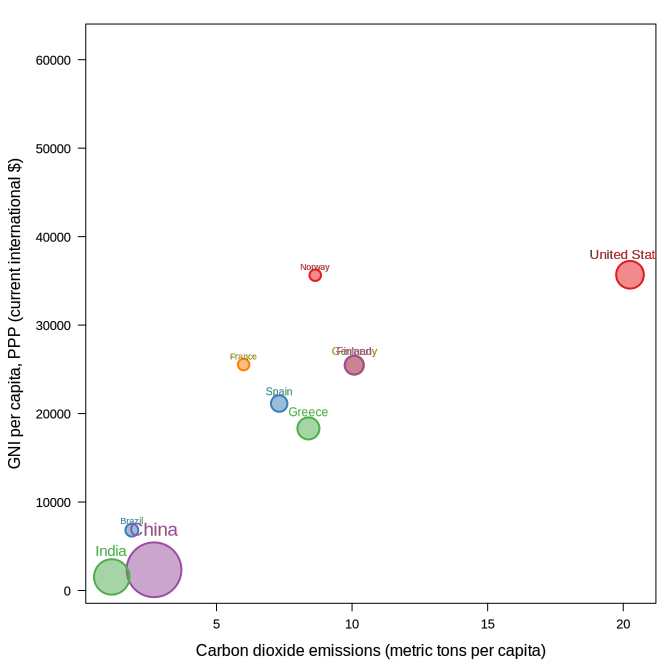
\includegraphics[width=\textwidth]{figs/bubbles.png}
  \caption{Animated bubbles produced with \texttt{gridSVG}.}
  \label{fig:bubblesSVG}
\end{figure}

Now, sit down in your favorite easy chair and watch the magistral
video ``200 Countries, 200 Years, 4 Minutes''\footnote{\url{http://www.gapminder.org/videos/200-years-that-changed-the-world-bbc/}}. After that, you are
ready to open the SVG file of traveling bubbles: It is easier, a short
time period with less than twenty countries.
